\section{Componentes Conectados}

\begin{frame}[fragile]{Conectividade de um grafo}

    \begin{itemize}
        \item Um grafo $G$ é dito conectado se, para qualquer par de vértices $u, v\in G$, com
            $u\neq v$, existe ao menos um caminho de $u$ até $v$

        \item Uma maneira de se verificar se um grafo é conectado ou não é iniciar uma travessia
            em um vértice $s$ qualquer

        \item Se a travessia visitar todos os $N$ nós de $G$ o grafo é conectado

        \item Caso um ou mais vértices não seja visitado, os nós visitados formam um 
            componente conectado de $G$

        \item Para identificar todos os componentes conectados do grafo basta iniciar uma nova
            travessia em um dos vértices não visitados, enquanto houverem vértices não
            visitados
    \end{itemize}

\end{frame}

\begin{frame}[fragile]{Visualização da identificação dos componentes conectados}

    \begin{tikzpicture}
        \draw (0,5) -- (2,9);
        \draw (0,5) -- (8,7);
        \draw (2,9) -- (10,8);
        \draw (2,2) -- (8,2);
        \draw (4,4) -- (6,8);
        \draw (4,4) -- (8,5);
        \draw (6,8) -- (8,5);

        \node[circle, draw, fill=white] at (0, 5) {1};
        \node[circle, draw, fill=white] at (2, 9) {2};
        \node[circle, draw, fill=white] at (2, 2) {3};
        \node[circle, draw, fill=white] at (4, 4) {4};
        \node[circle, draw, fill=white] at (6, 8) {5};
        \node[circle, draw, fill=white] at (6, 3) {6};
        \node[circle, draw, fill=white] at (8, 2) {7};
        \node[circle, draw, fill=white] at (8, 7) {8};
        \node[circle, draw, fill=white] at (8, 5) {9};
        \node[circle, draw, fill=white] at (10, 8) {10};

    \end{tikzpicture}

\end{frame}

\begin{frame}[fragile]{Visualização da identificação dos componentes conectados}

    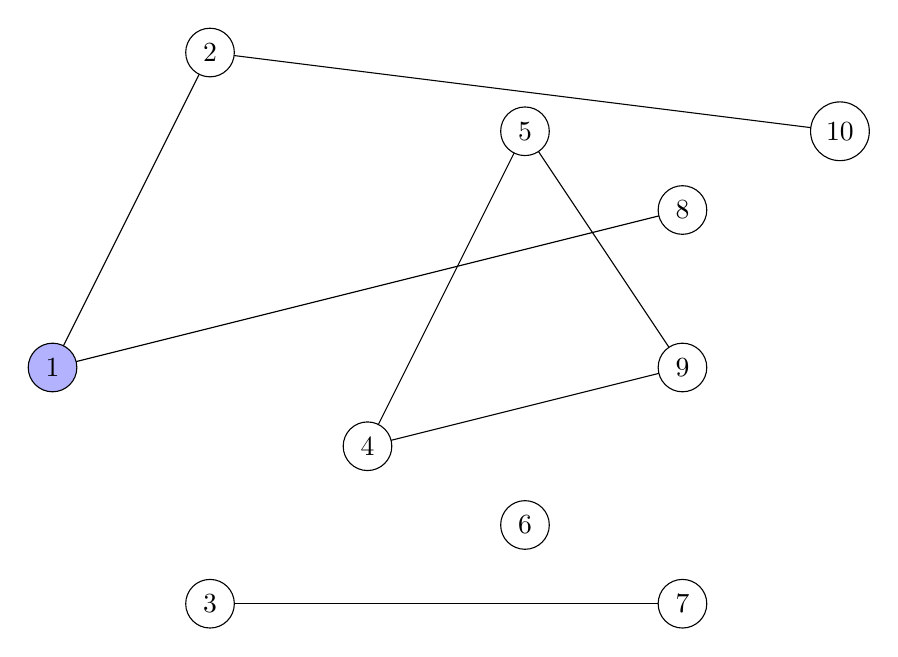
\begin{tikzpicture}
        \draw (0,5) -- (2,9);
        \draw (0,5) -- (8,7);
        \draw (2,9) -- (10,8);
        \draw (2,2) -- (8,2);
        \draw (4,4) -- (6,8);
        \draw (4,4) -- (8,5);
        \draw (6,8) -- (8,5);

        \node[circle, draw, fill=blue!30] at (0, 5) {1};
        \node[circle, draw, fill=white] at (2, 9) {2};
        \node[circle, draw, fill=white] at (2, 2) {3};
        \node[circle, draw, fill=white] at (4, 4) {4};
        \node[circle, draw, fill=white] at (6, 8) {5};
        \node[circle, draw, fill=white] at (6, 3) {6};
        \node[circle, draw, fill=white] at (8, 2) {7};
        \node[circle, draw, fill=white] at (8, 7) {8};
        \node[circle, draw, fill=white] at (8, 5) {9};
        \node[circle, draw, fill=white] at (10, 8) {10};

    \end{tikzpicture}

\end{frame}

\begin{frame}[fragile]{Visualização da identificação dos componentes conectados}

    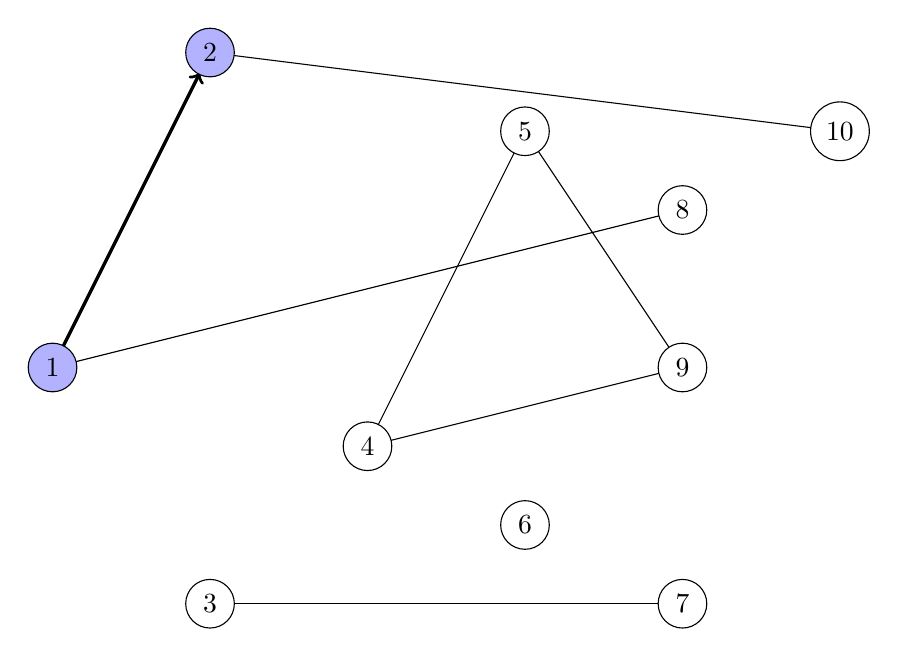
\begin{tikzpicture}
        \draw[very thick,->] (0,5) -- (1.87,8.74);
        \draw (0,5) -- (8,7);
        \draw (2,9) -- (10,8);
        \draw (2,2) -- (8,2);
        \draw (4,4) -- (6,8);
        \draw (4,4) -- (8,5);
        \draw (6,8) -- (8,5);

        \node[circle, draw, fill=blue!30] at (0, 5) {1};
        \node[circle, draw, fill=blue!30] at (2, 9) {2};
        \node[circle, draw, fill=white] at (2, 2) {3};
        \node[circle, draw, fill=white] at (4, 4) {4};
        \node[circle, draw, fill=white] at (6, 8) {5};
        \node[circle, draw, fill=white] at (6, 3) {6};
        \node[circle, draw, fill=white] at (8, 2) {7};
        \node[circle, draw, fill=white] at (8, 7) {8};
        \node[circle, draw, fill=white] at (8, 5) {9};
        \node[circle, draw, fill=white] at (10, 8) {10};

    \end{tikzpicture}

\end{frame}

\begin{frame}[fragile]{Visualização da identificação dos componentes conectados}

    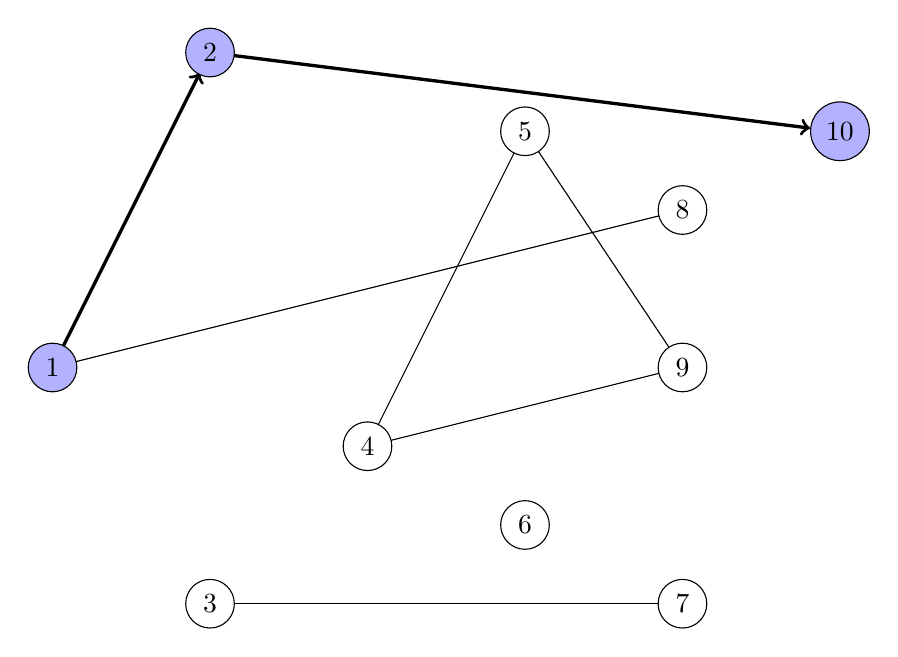
\begin{tikzpicture}
        \draw[very thick,->] (0,5) -- (1.87,8.74);
        \draw (0,5) -- (8,7);
        \draw[very thick,->] (2,9) -- (9.62,8.04);
        \draw (2,2) -- (8,2);
        \draw (4,4) -- (6,8);
        \draw (4,4) -- (8,5);
        \draw (6,8) -- (8,5);

        \node[circle, draw, fill=blue!30] at (0, 5) {1};
        \node[circle, draw, fill=blue!30] at (2, 9) {2};
        \node[circle, draw, fill=white] at (2, 2) {3};
        \node[circle, draw, fill=white] at (4, 4) {4};
        \node[circle, draw, fill=white] at (6, 8) {5};
        \node[circle, draw, fill=white] at (6, 3) {6};
        \node[circle, draw, fill=white] at (8, 2) {7};
        \node[circle, draw, fill=white] at (8, 7) {8};
        \node[circle, draw, fill=white] at (8, 5) {9};
        \node[circle, draw, fill=blue!30] at (10, 8) {10};

    \end{tikzpicture}

\end{frame}

\begin{frame}[fragile]{Visualização da identificação dos componentes conectados}

    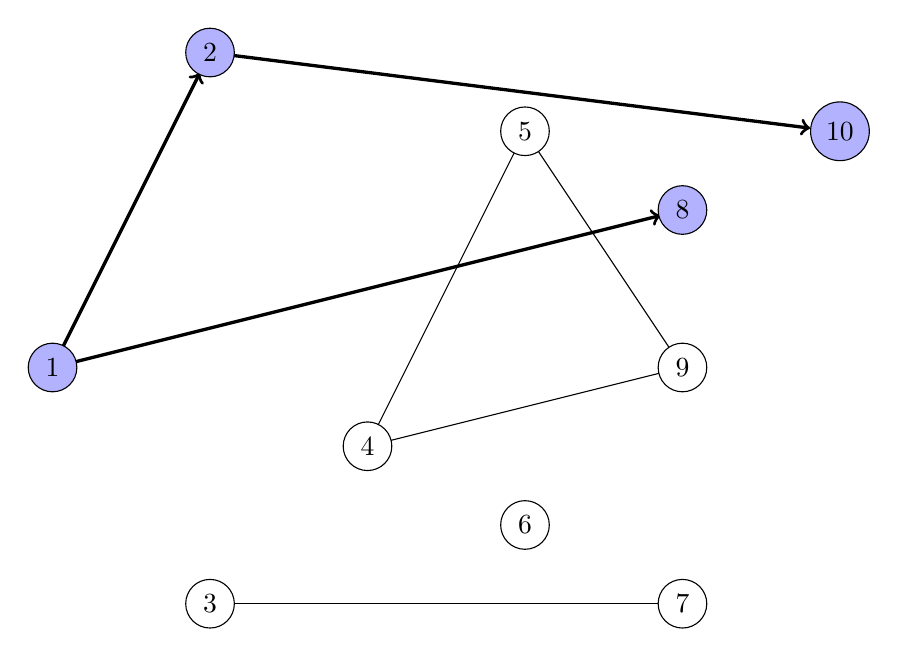
\begin{tikzpicture}
        \draw[very thick,->] (0,5) -- (1.87,8.74);
        \draw[very thick,->] (0,5) -- (7.72,6.93);
        \draw[very thick,->] (2,9) -- (9.62,8.04);
        \draw (2,2) -- (8,2);
        \draw (4,4) -- (6,8);
        \draw (4,4) -- (8,5);
        \draw (6,8) -- (8,5);

        \node[circle, draw, fill=blue!30] at (0, 5) {1};
        \node[circle, draw, fill=blue!30] at (2, 9) {2};
        \node[circle, draw, fill=white] at (2, 2) {3};
        \node[circle, draw, fill=white] at (4, 4) {4};
        \node[circle, draw, fill=white] at (6, 8) {5};
        \node[circle, draw, fill=white] at (6, 3) {6};
        \node[circle, draw, fill=white] at (8, 2) {7};
        \node[circle, draw, fill=blue!30] at (8, 7) {8};
        \node[circle, draw, fill=white] at (8, 5) {9};
        \node[circle, draw, fill=blue!30] at (10, 8) {10};

    \end{tikzpicture}

\end{frame}

\begin{frame}[fragile]{Visualização da identificação dos componentes conectados}

    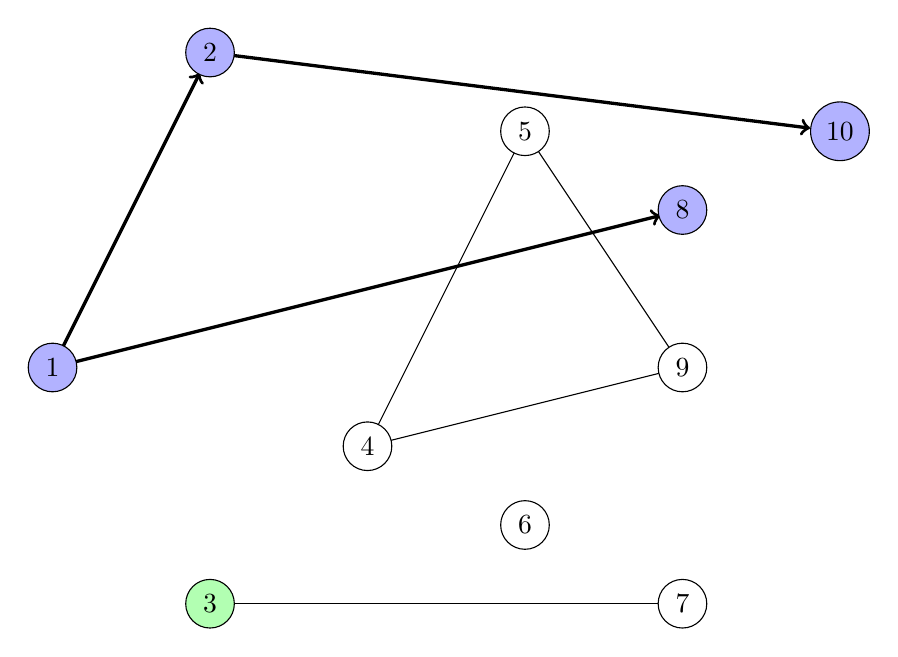
\begin{tikzpicture}
        \draw[very thick,->] (0,5) -- (1.87,8.74);
        \draw[very thick,->] (0,5) -- (7.72,6.93);
        \draw[very thick,->] (2,9) -- (9.62,8.04);
        \draw (2,2) -- (8,2);
        \draw (4,4) -- (6,8);
        \draw (4,4) -- (8,5);
        \draw (6,8) -- (8,5);

        \node[circle, draw, fill=blue!30] at (0, 5) {1};
        \node[circle, draw, fill=blue!30] at (2, 9) {2};
        \node[circle, draw, fill=green!30] at (2, 2) {3};
        \node[circle, draw, fill=white] at (4, 4) {4};
        \node[circle, draw, fill=white] at (6, 8) {5};
        \node[circle, draw, fill=white] at (6, 3) {6};
        \node[circle, draw, fill=white] at (8, 2) {7};
        \node[circle, draw, fill=blue!30] at (8, 7) {8};
        \node[circle, draw, fill=white] at (8, 5) {9};
        \node[circle, draw, fill=blue!30] at (10, 8) {10};

    \end{tikzpicture}

\end{frame}
